%!TEX root = ../acc-optim.tex
\section{Array fusion} % (fold)
\label{sec:fusion}

\begin{figure}
\flushright
\small(Before fusion)\qquad\\
\centering
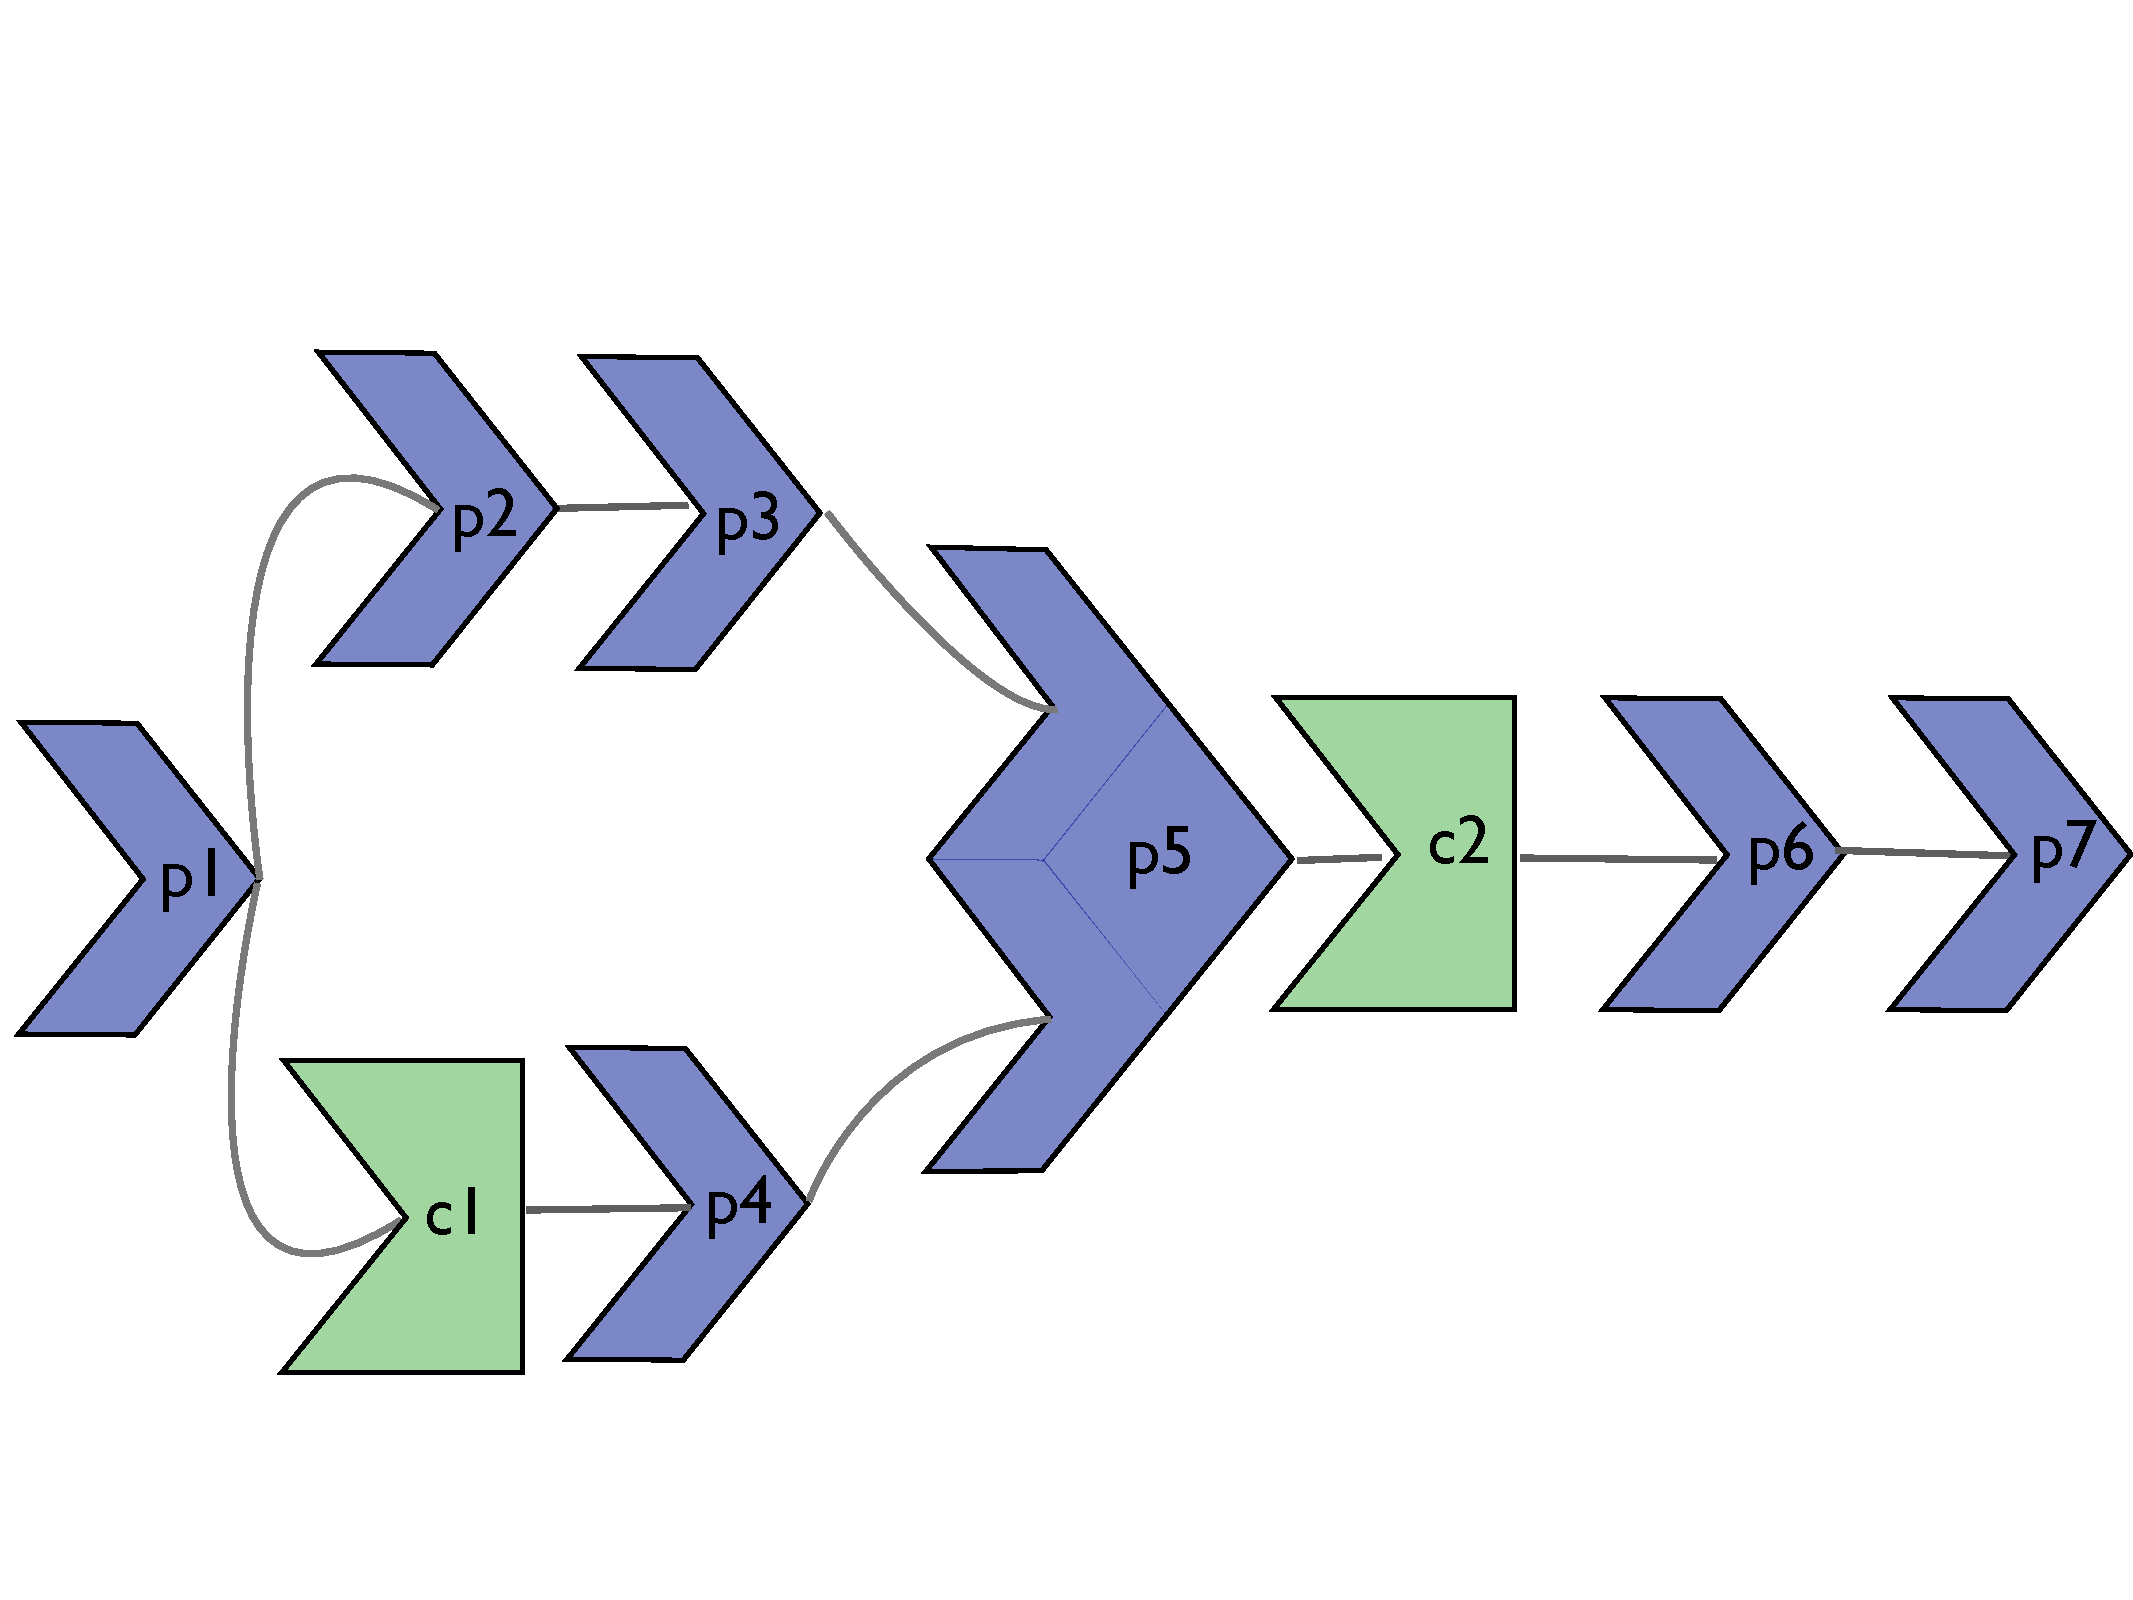
\includegraphics[scale=0.175]{figs/fusion1.pdf}
\flushright
\small(After producer/producer fusion)\qquad\\
\centering
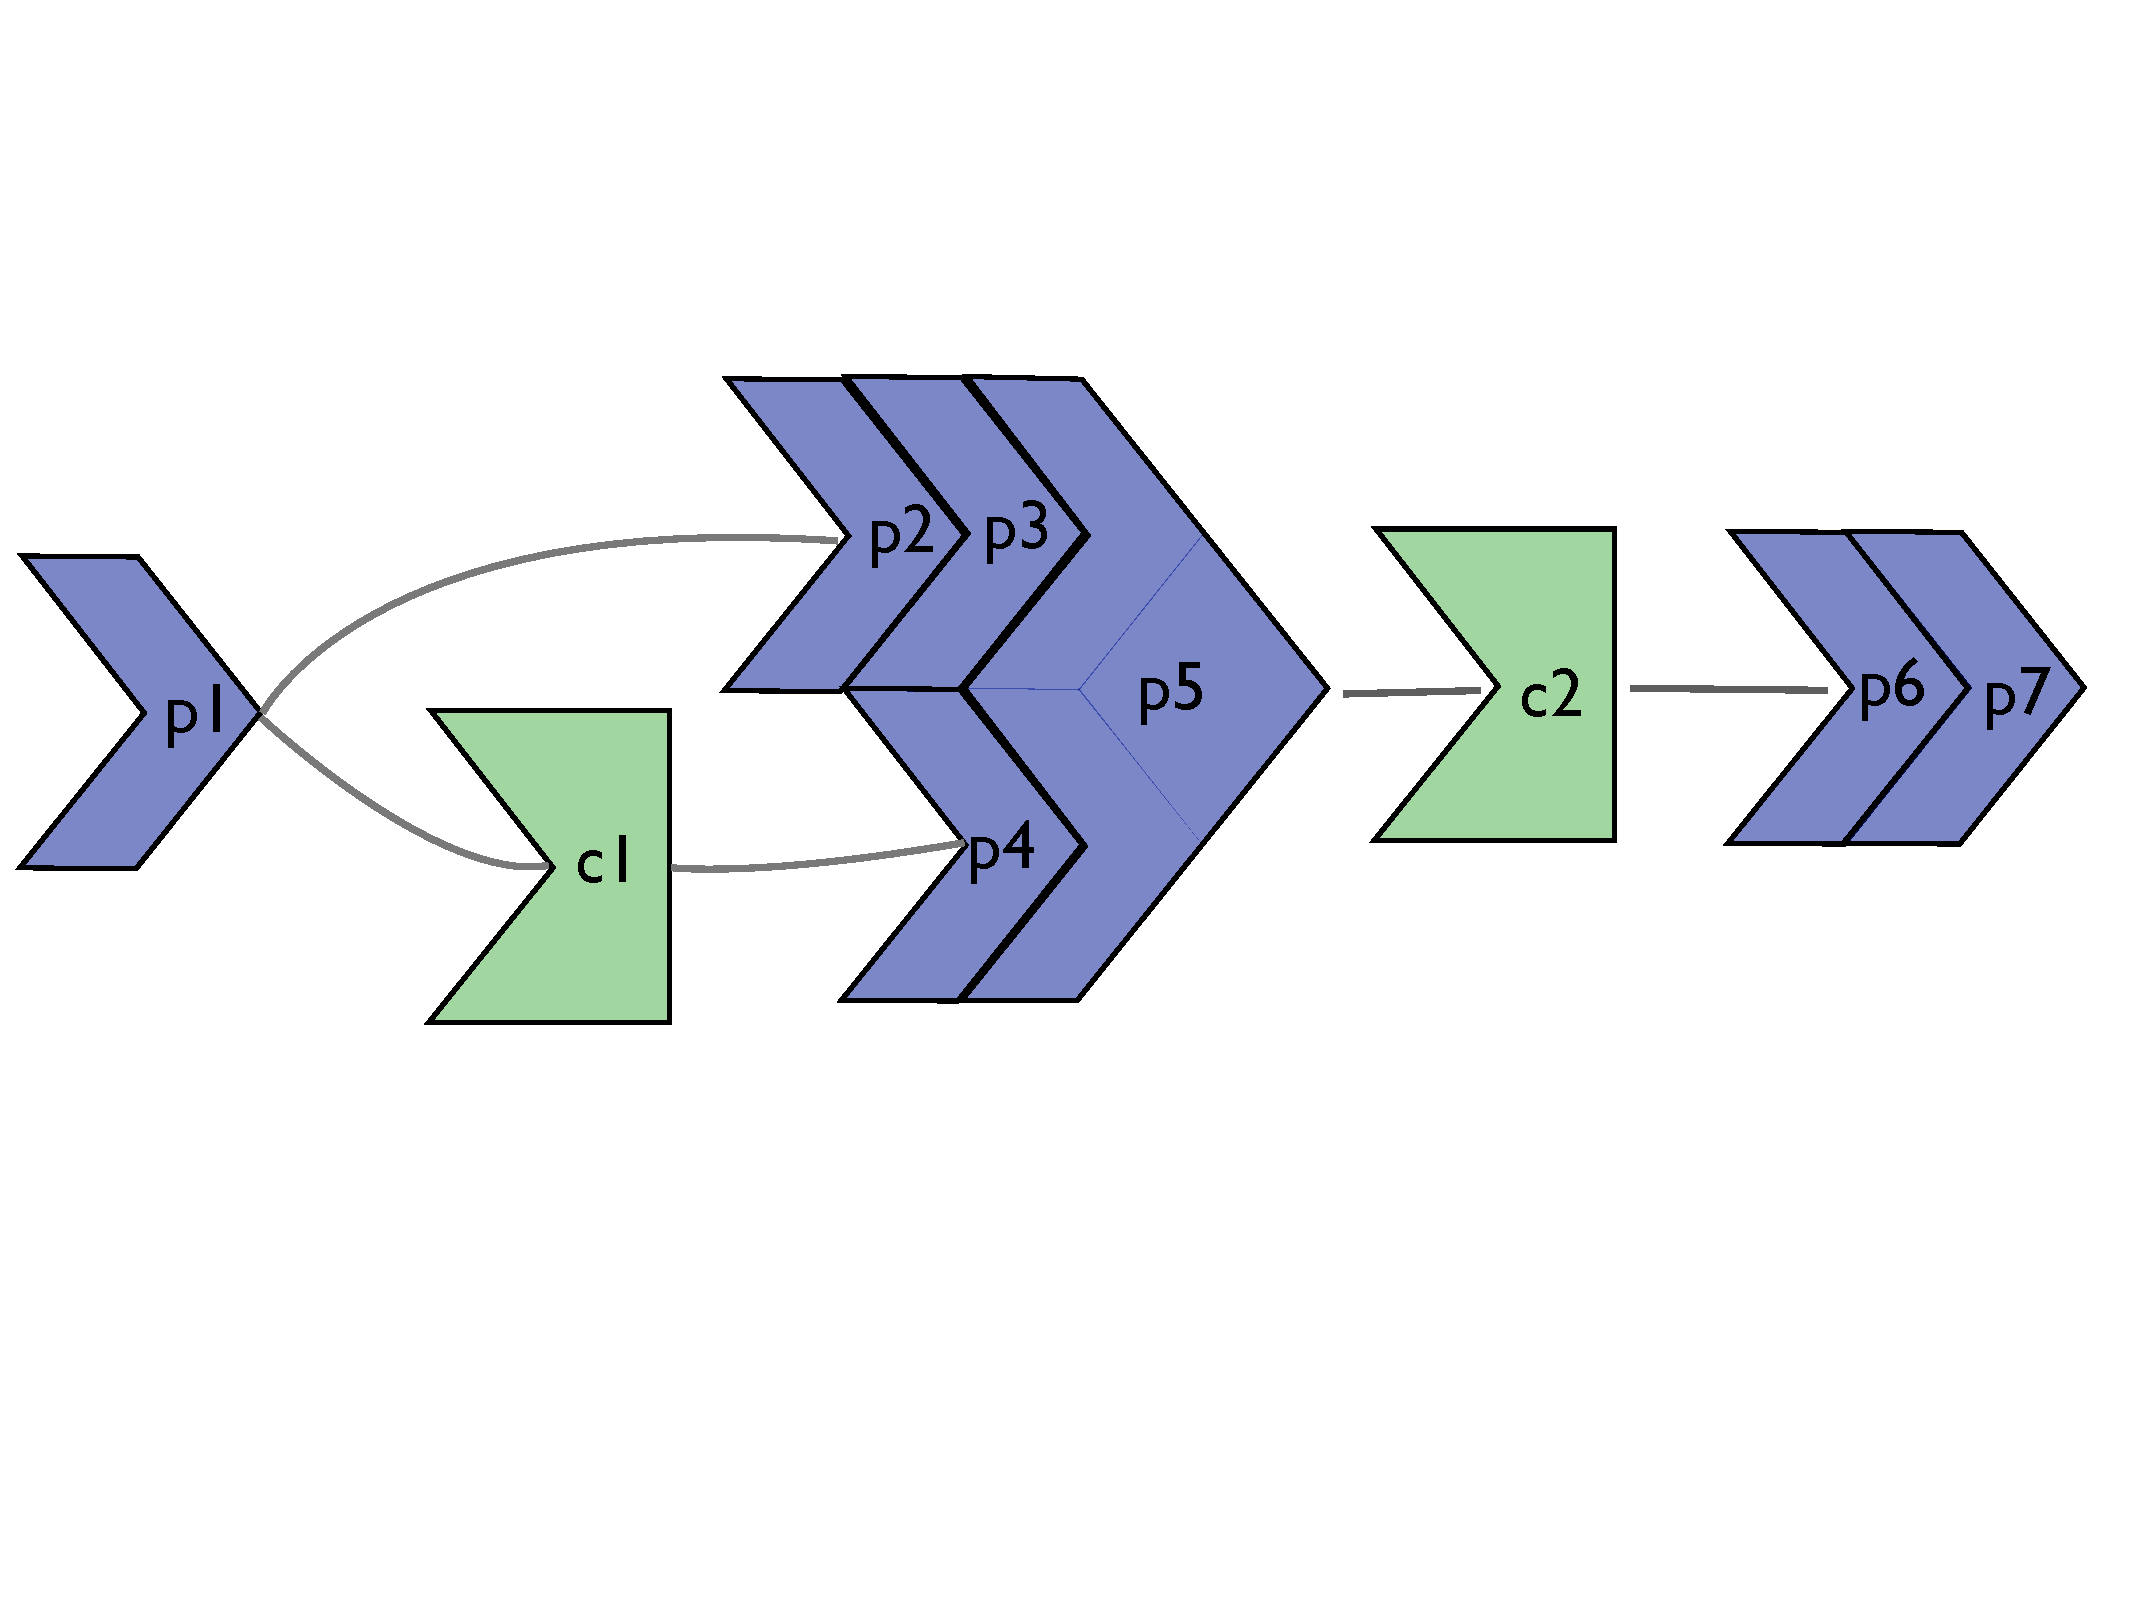
\includegraphics[scale=0.175]{figs/fusion2.pdf}
\flushright
\small(After consumer/producer fusion)\qquad\\
\centering
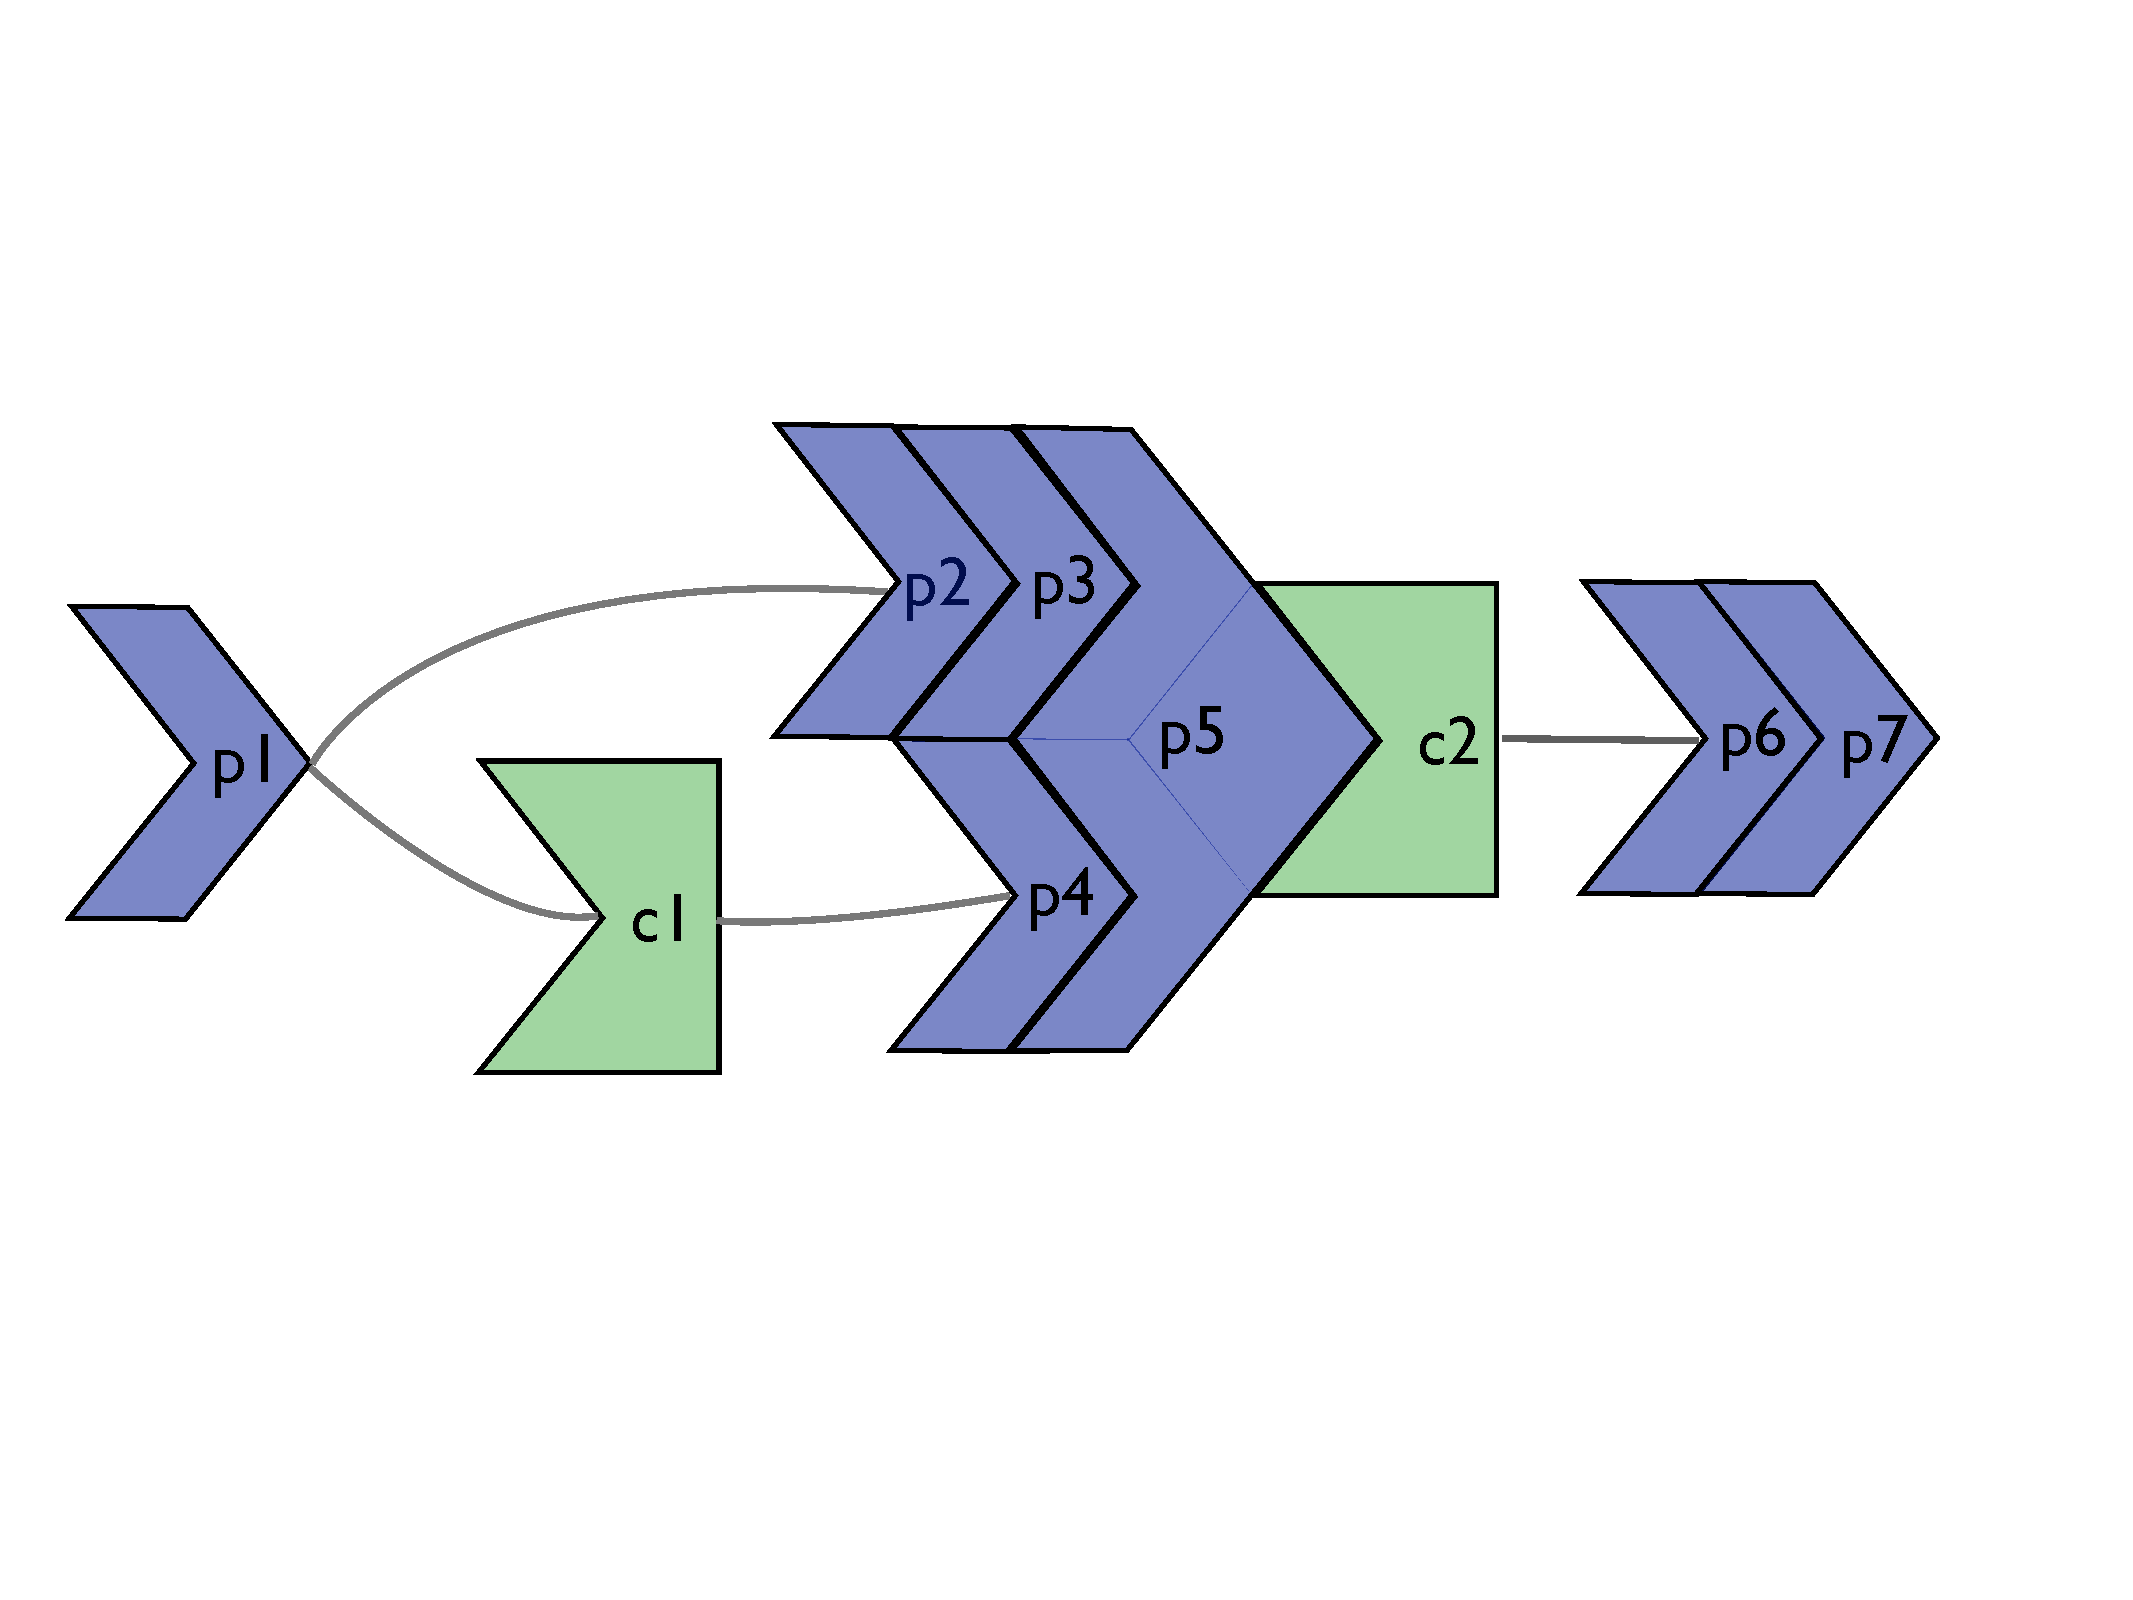
\includegraphics[scale=0.175]{figs/fusion3.pdf}
\caption{Produce/producer and consumer/producer fusion}
\label{fig:Fusion}
\end{figure}

Fusion in a massively data-parallel, embedded language for GPUs, such as Accelerate, requires a few uncommon considerations.

\paragraph{Parallelism.} While fusing parallel collective operations, we must be careful not to lose information essential to parallel execution. For example, \texttt{foldr/build} fusion \cite{Gill:1993de} is not applicable, because it produces sequential tail-recursive loops rather than massively parallel GPU kernels. Similarly, the \texttt{split/join} approach used in Data Parallel Haskell (DPH)~\cite{Keller:distributed-types} is not helpful, although fused operations are split into sequential and parallel subcomputations, as they assume an explicit parallel scheduler, which in DPH is written directly in Haskell. Accelerate compiles massively parallel array combinators to CUDA code via template skeleton instantiation, so any fusion system must preserve the combinator representation of the intermediate code. 

\paragraph{Sharing.} Existing fusion transforms rely on inlining to move producer and consumer expressions next to each other, which allows producer/consumer pairs to be detected. However, when let-bound variables are used multiple times in the body of an expression, unrestrained inlining can lead to duplication of work. Compilers such as GHC, handle this situation by only inlining the definitions of let-bound variables that have a single use site, or by relying on some heuristic about the size of the resulting code to decide what to inline \cite{PeytonJones:Inliner}. However, in typical Accelerate programs, each array is used at least twice: once to access the shape information and once to access the array data; so, we must handle at least this case separately.

\paragraph{Filtering.} General array fusion transforms must deal with filter-like operations, for which the size of the result structure depends on the \emph{value} of the input structure, as well as its size. Accelerate does not encode filtering as a primitive operation, so we do not need to consider it further.\footnote{@filter@ is easily implemented as a combination of the core primitives, and is provided as part of the library.}

\paragraph{Fusion at run-time.}
As the Accelerate language is embedded in Haskell, compilation of the Accelerate program happens at Haskell \emph{runtime} rather than when compiling the Haskell program. For this reason, optimisations applied to an Accelerate program contribute to its overall runtime, so we must be mindful of the cost of analysis and code transformation. On the flip-side, runtime optimisations can make use of information that is only available at runtime. 

\paragraph{Fusion on typed de Brujin terms.}
We fuse Accelerate programs by rewriting typed de Bruijn terms in a type preserving manner. However, maintaining type information adds complexity to the definitions and rules, which amounts to a partial proof of correctness checked by the type checker, but is not particularly exciting for the present exposition. Hence, in this section, we elide the steps necessary to maintain type information during fusion.

\begin{table*}
\begin{lstlisting}[escapechar={\%}]
%\makebox[\textwidth]{\rm\bf Producers}%
map         :: (Exp a -> Exp b) -> Acc (Array sh a) -> Acc (Array sh b)             %\rm map a function over an array%
zipWith     :: (Exp a -> Exp b -> Exp c) -> Acc (Array sh a) -> Acc (Array sh b)    %\rm apply funciton to\ldots%
            -> Acc (Array sh c)                                                     %\rm \ldots a pair of arrays%
backpermute :: Exp sh' -> (Exp sh' -> Exp sh) -> Acc (Array sh a)                   %\rm backwards permutation%
            -> Acc (Array sh' e)
replicate   :: Slice slix => Exp slix                                               %\rm extend array across\ldots%
            -> Acc (Array (SliceShape slix) e)                                      %\rm \ldots new dimensions%
            -> Acc (Array (FullShape  slix) e)
slice       :: Slice slix                                                           %\rm remove existing dimensions%
            => Acc (Array (FullShape  slix) e) -> Exp slix
            -> Acc (Array (SliceShape slix) e)
generate    :: Exp sh -> (Exp sh -> Exp a) -> Acc (Array sh a)                      %\rm array from index mapping%

%\makebox[\textwidth]{\rm\bf Consumers}%
fold        :: (Exp a -> Exp a -> Exp a) -> Exp a -> Acc (Array (sh:.Int) a)        %\rm tree reduction along\ldots%
            -> Acc (Array sh a)                                                     %\rm \ldots innermost dimension%
scan{l,r}   :: (Exp a -> Exp a -> Exp a) -> Exp a -> Acc (Vector a)                 %\rm left-to-right or right-to-left%
            -> Acc (Vector a)                                                       %\rm \ldots vector pre-scan%
permute     :: (Exp a -> Exp a -> Exp a) -> Acc (Array sh' a)                       %\rm forward permutation%
            -> (Exp sh -> Exp sh') -> Acc (Array sh a) -> Acc (Array sh' a)
stencil     :: Stencil sh a stencil => (stencil -> Exp b) -> Boundary a             %\rm map a function with local\ldots%
            -> Acc (Array sh a) -> Acc (Array sh b)                                 %\rm \ldots neighbourhood context%
\end{lstlisting}
\caption[Core Accelerate array operations]{Summary of Accelerate's core
    collective array operations, omitting \texttt{Shape} and \texttt{Elt}
    class constraints for brevity. In addition, there are other flavours of
    folds and scans as well as segmented versions of these.}
\label{tab:operations}
\end{table*}


% -----------------------------------------------------------------------------
\subsection{The Main Idea}
All collective operations in Accelerate are array-to-array transformations. Reductions, such as \texttt{fold}, which reduce an array to a single element, yield a singleton array rather than a scalar expression. Hence, we can partition array operations into two categories:
%
\begin{enumerate}
\item Operations where each element of the result array depends on at most one element of each input array. Multiple elements of the output array may depend on a single input array element, but all output elements can be computed independently. We refer to these operations as \textit{producers}.

\item Operations where each element of the result array depends on multiple elements of the input array. We call these functions \textit{consumers}, in spite of the fact that they also produce an array.
\end{enumerate}
%
Table~\ref{tab:operations} summarises the collective array operations that we support. In a parallel context, producers are more pleasant to deal with because independent element-wise operations have an obvious mapping to the GPU. Consumers are a different story, as we need to know exactly how the computations depend on each other to implement them efficiently. For example, a parallel fold (with an associative operator) can be implemented efficiently as a tree reduction, but a parallel scan requires two separate phases \cite{Sengupta:2007tc, Chatterjee:1990vj}. Unfortunately, this sort of information is obfuscated by most fusion techniques. To support the different properties of producers and consumers, our fusion transform is split into two distinct phases:
%
\begin{itemize}
\item \emph{Producer/producer:} fuse sequences of producers into a single producer. This is implemented as a source-to-source transformation on the AST.

\item \emph{Consumer/producer:} fuse producers followed by a consumer into the consumer. This happens during code generation, where we specialise the consumer skeleton with the producer code.
\end{itemize}
%
Separating fusion into these two phases reduces the complexity of the task, though there is also a drawback: as all collective operations in Accelerate output arrays, we might wish to use the output of a consumer as an input to a producer as in @map g . fold f z@. Here, the \texttt{map} operation could be fused into the \texttt{fold} by applying the function \texttt{g} to each element produced by the reduction before storing the final result in memory. This is useful, as Accelerate works on multidimensional arrays, so the result of a \texttt{fold} can be a large array rather than just a singleton array. Our approach currently does not fuse producer/consumer pairs, only consumer/producer and producer/producer combinations. 

Figure~\ref{fig:Fusion} illustrates how fusion affects the AST: blue boxes $p_1$ to $p_7$ represent producers, where $p_5$ is a producer like \texttt{zipWith} with two input arrays. The consumers are $c_1$ and $c_2$. Firstly, we fuse all producers, with the exception of $p_1$ whose result is used by both $c_1$ and $p_2$. Next, we plug the fused producers into consumers where possible. Again, $p_1$ is left as is. It would be straightforward to change our implementation such that it would fuse $p_1$ into both $p_2$ and $c_1$. This would duplicate the work of $p_1$ into both $p_2$ and $c_1$, which, despite reducing memory traffic, is not always advantageous. Our current implementation is conservative and never duplicates work; we plan to change this in future work as the restricted nature of Accelerate means that we can compute accurate cost estimates and make an informed decision. In contrast, producer/consumer fusion of $c_1$ into $p_4$ would require fundamental changes.


% -----------------------------------------------------------------------------
\subsection{Producer/producer fusion for parallel arrays}

The basic idea behind the representation of producer arrays in Accelerate is well known: simply represent an array by its shape and a function mapping indices to their corresponding values. We previously used it successfully to optimise purely functional array programs in Repa~\cite{Keller:Repa}, but it was also used by others~\cite{Claessen:obsidian-expressive}.

However, there are at least two reasons why it is not always beneficial to represent all array terms uniformly as functions. One is \emph{sharing}: we must be able to represent some terms as manifest arrays so that a delayed-by-default representation can not lead to arbitrary loss of sharing. This is a well known problem in Repa. The other consideration is \emph{efficiency}: since we are targeting an architecture designed for performance, we prefer more specific operations. An opaque indexing function is too general, conveying no information about the pattern in which the underlying array is accessed, and hence no opportunities for optimisation. We shall return to this point in Section~\ref{sec:benchmarks}, but already include a form of structured traversal over an array (@Step@) in the following definition:

% It is parametrised with the shape of the result array, a function which, given
% an index in the result array, returns an index into the manifest source array
% argument.
\begin{code}
  data DelayedAcc a where
    Done  :: Acc a
          -> DelayedAcc a

    Yield :: (Shape sh, Elt e)
          => Exp sh
          -> Fun (sh -> e)
          -> DelayedAcc (Array sh e)

    Step  :: (Shape sh, Shape sh', Elt e, Elt e')
          => Exp sh'
          -> Fun (sh' -> sh)
          -> Fun (e -> e')
          -> Idx (Array sh e)
          -> DelayedAcc (Array sh' e')
\end{code}
%
We have three constructors: \texttt{Done} injects a manifest array into the
type. \texttt{Yield} defines a delayed array in terms of its shape and a
function which maps indices to elements. The third constructor, \texttt{Step},
encodes a special case of the more general \texttt{Yield} that represents the
application of an index and/or value space transformation to the argument array.
The type \texttt{Fun (sh -> e)} is that of a term representing a scalar
function from shape to element type. The type \texttt{Idx (Array sh e)} is that of a de
Bruijn index representing an array valued variable. Representing the argument
array in this way means that both \texttt{Step} and \texttt{Yield} are
non-recursive in \texttt{Acc} terms, and so they can always be expressed as
scalar functions and embedded into consumers in the second phase of fusion.

We represent all array functions as constructors of the type \texttt{DelayedAcc}. Producer/producer fusion is achieved by tree contraction on the AST, merging sequences of producers into a single one. All array producing functions, such as \texttt{map} and \texttt{backpermute}, are expressed in terms of smart constructors for the \texttt{DelayedAcc} type. The smart constructors manage the integration with successive producers, as shown in the following definition of \texttt{mapD}, the delayed version of the \texttt{map} function:
%
\begin{code}
  mapD :: (Shape sh, Elt a, Elt b)
       => Fun (a -> b)
       -> DelayedAcc (Array sh a)
       -> DelayedAcc (Array sh b)
  mapD f (Step  sh p g v) = Step  sh p (f . g) v
  mapD f (Yield sh g)     = Yield sh   (f . g)
\end{code}
%
The function composition operator \texttt{(.)} is overloaded here to work on scalar function terms. With this definition we now have the well known fusion rule that reduces \texttt{mapD f . mapD g} sequences to \texttt{mapD (f . g)}. Similarly, the definition of delayed backpermute means that \mbox{\texttt{backpermuteD sh p (backpermuteD \_ q arr)}} reduces to \texttt{backpermute sh (q . p) arr}:
\begin{code}
backpermuteD
    :: (Shape sh, Shape sh', Elt e)
    => Exp        sh'
    -> Fun        (sh' -> sh)
    -> DelayedAcc (Array sh  e)
    -> DelayedAcc (Array sh' e)
backpermuteD sh' p acc = case acc of
  Step  _ ix f a  -> Step  sh' (ix . p) f a
  Yield _ f       -> Yield env sh' (f . p)
  Done  env a     -> Step  sh' p identity (toIdx a)
\end{code}
% \gck{Manuel: as discussed, we may have to put in the valuation. Does backpermute really add anything here anyway?}
Of course, combinations of maps with backpermutes also reduce to a single producer. %, albeit one that does not correspond to one of the Accelerate built-in array operations.

As desired, this approach also works on producers which\linebreak
take their input from multiple arrays. This is in contrast to\linebreak
\texttt{foldr/build}~\cite{Gill:1993de}, which
can fuse one of the input arguments, but not both. The definition of \texttt{zipWithD} considers 
all possible combinations of constructors (only some of which we list here) and can therefore fuse producers of both arguments:
%
\begin{code}
  zipWithD :: (Shape sh, Elt a, Elt b, Elt c)
           => Fun (a -> b -> c)
           -> DelayedAcc (Array sh a)
           -> DelayedAcc (Array sh b)
           -> DelayedAcc (Array sh c)
  zipWithD f (Yield sh1 g1) (Yield sh2 g2)
    = Yield (sh1 `intersect` sh2)
            (\sh -> f (g1 sh) (g2 sh))
  zipWithD f (Yield sh1 g1) (Step  sh2 ix2 g2 a2)
    = Yield ...
\end{code}
%
In this manner, sequences of producers fuse into a single producer term; then, we turn them back into a manifest array using the function \texttt{compute}. It inspects the argument terms of the delayed array to identify special cases, such as maps or backpermutes, as shown in the following snippet of pseudo-code:
%
\begin{code}
  compute :: DelayedAcc a -> Acc a
  compute (Done a)          = a
  compute (Yield sh f)      = Generate sh f
  compute (Step sh p f v)
    | sh == shape a, isId p, isId f 
                            = a
    | sh == shape a, isId p = Map f a
    | isId f                = Backpermute sh p a
    | otherwise             = Transform sh p f a
    where a = Avar v
\end{code}
%
Since we operate directly on the AST of the program, we can inspect function arguments and specialise the code accordingly. For example, \texttt{isId :: Fun (a->b) -> Bool} checks whether a function term corresponds to the term $\lambda x. x$. 


% -----------------------------------------------------------------------------
\subsection{Consumer/Producer Fusion}
Now that we have the story for producer/producer fusion, we discuss how to deal with consumers. We pass producers encoded in the @DelayedAcc@ representation as arguments to consumers, so that the consumers can compute the elements they need on-the-fly. Consumers themselves have no @DelayedAcc@ representation, however.

Consumers such as \texttt{stencil}, access elements of their argument array multiple times. These consumers are implemented carefully not to duplicate work. Indeed, even when the argument of such a consumer is a manifest array, the consumer should ensure that it caches already fetched elements, as GPUs impose a high performance penalty for repeated memory loads. Some consumers can be implemented more efficiently when given a producer expressed in terms of a function from a multi-dimensional array index to an element value. Other consumers prefer functions that map the flat linear index of the underling array to its value. Our consumer-friendly representation of delayed arrays therefore contains both versions: 
%
\begin{code}
data Embedded sh e
  =  (Shape sh, Elt e) 
  => DelayedArray { extent      :: Exp sh
                  , index       :: Fun (sh  -> e)
                  , linearIndex :: Fun (Int -> e) }

embedAcc :: (Shape sh, Elt e) 
         => Acc (Array sh e) -> Embedded sh e
embedAcc (Generate sh f)  
  = DelayedArray sh f (f . (fromIndex sh))
embedAcc (Map f (AVar v)) 
  = DelayedArray (shape v) (indexArray v) 
                           (linearIndexArray v)
embedAcc ...
\end{code}
%
The function \texttt{embedAcc} intelligently injects each producer into the \texttt{Embedded} type by inspection of the constructor, as shown in the code snippet above. In theory, \texttt{compute} and \texttt{embedAcc} could be combined to go directly from the delayed representation which is convenient for producer/producer fusion to the one for consumer/producer fusion. However, these two steps happen at different phases in the compilation, so we want to limit the visibility of each delayed representation to the current phase.

Producers are finally embedded into consumers during code generation. During code generation, the code for the embedded producers is plugged into the consumer template. The \texttt{codegenAcc} function inspects the consumer and generates code for the arguments of the consumer. It then passes these CUDA code snippets to a function specialised on generating code for this particular consumer (\texttt{mkFold} in the example below), which combines these snippets with the actual CUDA consumer code:
\begin{code}
 codegenAcc :: DeviceProperties -> OpenAcc arrs 
            -> Gamma aenv -> CUTranslSkel arrs 
 codegenAcc dev (OpenAcc (Fold f z a)) aenv 
   = mkFold dev  aenv (codeGenFun f) (codeGenExp z) 
            (codegenDelayedAcc $ embedAcc a)
 codegenAcc dev (OpenAcc (Scanl f z a)) aenv 
   = ...
\end{code}
%
As a result, the code producing each element is integrated directly into the consumer, and no intermediate array needs to be created.


% -----------------------------------------------------------------------------
\subsection{Exploiting all opportunities for fusion}

As mentioned previously, we need to be careful about fusing shared array computations, to avoid duplicating work. However, \emph{scalar} Accelerate computations that manipulate \emph{array shapes}, as opposed to the bulk array data, can lead to terms that employ sharing, but can never duplicate work. Such terms are common in Accelerate code, and it is important to that they do not inhibit fusion.

Consider the following example that first reverses a vector with @backpermute@ and then maps a function @f@ over the result. Being a sequence of two producer operations, we would hope these are fused into a single operation:
%
\begin{code}
  reverseMap f a
    = map f
    $ backpermute (shape a) (\i->length a-i-1) a
\end{code}
%
Unfortunately, sharing recovery, using the algorithm from Section~\ref{sec:sharing}, causes a problem. The variable @a@ is used three times in the arguments to @backpermute@; hence, sharing recovery will introduce a let binding at the lowest common meet point for all uses of the array. This places it between the \texttt{map} and \texttt{backpermute} functions:
%
\begin{code}
  reverseMap f a
    = map f
    $ let v = a
      in backpermute (shape v) (\i->length v-i-1) v
\end{code}
%
This binding, although trivial, prevents fusion of the two producers, and it does so unnecessarily. The argument array is used three times: twice to access shape information, but only once to access the array data --- in the final argument to \texttt{backpermute}. 

Fortunately, there is a simple work around. Recall that our delayed array constructors \texttt{Step} and \texttt{Yield} carry the shape of the arrays they represent. Hence, we can eliminate all uses of the array that \emph{only access shape information}, leaving us with a single reference to the array's payload. That single reference enables us to remove the let binding and to re-enable fusion.

Similarly, we may float let bindings of manifest data out (across producer chains). This helps to expose further opportunities for producer/producer fusion. For example, we allow the binding of \texttt{xs} to float above the \texttt{map} so the two producers can be fused:
%
\begin{code}
  map g $ let xs = use (Array ...)
          in zipWith f xs xs
\end{code}

While floating let bindings opens up the potential for further optimisations, we are careful to not increase the lifetime of bound variables, as this would increase live memory usage.


% % -----------------------------------------------------------------------------
% \subsection{Hylomorphism Fusion}
% On a denotational level, our array fusion system is an instance of hylomorphism fusion as described by Takano and Meijer in \cite{Takano:shortcut-calculational}. Recall from \cite{Meijer:bananas} that a hylomorphism is a combination of an \emph{anamorphism} (unfold) that creates a bulk structure, followed by a \emph{catamorphism} (fold) that immediately reduces it. In \cite{Takano:shortcut-calculational} the ``bulk structures'' are presented as general F-algebras, and a third component gives a natural transformation between the input and output algebras. For the present discussion we can think of an F-algebra as an abstract data type, though see \cite{Takano:shortcut-calculational} for the formal definition. The three components of a hylomorphism are bundled together in ``envelope'' brackets which have the following signature.
% $$
% [\_, \_, \_]_{G,F} 
%         : \forall A B
%         . (G A \to A) \times (F \to G) \times (B \to F B)
%         \to (B \to A)
% $$

% For a given hylomorphism $[\varphi, \eta, \psi]$ the $\varphi$ is the catamorphism (fold) part, $\eta$ is the natural transformation, and $\psi$ is the anamorphism (unfold) part. 

% The @foldGen@ function described in \REF allows us to evaluated a restricted form of hylomorphism, namely one that can be efficiently computed on our parallel machine. 

% \begin{code}
%   foldGen :: Exp (sh :. Int) 
%           -> Fun ((sh :. Int) -> e)
%           -> Fun (e -> e -> e) 
%           -> Exp e 
%           -> Acc (Array sh e)
% \end{code}

% In @foldGen@, the first two arguments define the anamorphism (unfold), and the last two give the catamorphism (fold). Whereas the formal system of \cite{Takano:shortcut-calculational} expresses fusion over arbitrary data types, Accelerate only works on parallel arrays. In regards to the general definition, $B$ corresponds to array index @(sh :. Int)@ and $A$ corresponds to the result value @(Array sh e)@. The two functors $F$ and $G$ are fixed by the implementation. The object $F B$ is the function that takes each index and produces the element at that index @((sh:.Int) -> e)@. The object $G A$ corresponds to the intermediate array @(Array (sh:.Int) e)@ before it is reduced to @(Array sh e)@. The natural transformation performs the representation change between the two ``views'' of the intermediate array, that of a function that produces elements @((sh:.Int) -> e)@, and that of an indexable data structure @Array (sh:.Int) e@. The producer and consumer rules of \REF are then instances of the Cata-Hylo and Hylo-Ana fusion rules of   \cite{Takano:shortcut-calculational}.


% % -----------------------------------------------------------------------------
% \subsection{Hylomorphism fusion for parallel arrays}
% ... compare our instance of the anamorphism so the one from the standard Haskell library:

% @unfoldr :: (s -> (s, a)) -> s -> List a@

% In this case underlying functor $F$ provides a state parameter @s@ that is threaded through the computation. Although the state parameter allows the value of each successive element to depend on the previous one, it also makes the computation naturally sequential, so is not appropriate for our purposes.

% \ben{Say something about how @foldGen@ changes the index space from @(sh :. Int)@ to plain @sh@}.

% section fusion (end)
